\subsection{Retrival}

arXiv is the largest hub for open access scientific papers.
It also supports the Open Archives Initiative (OAI),
so a large volume of metadata can be easily downloaded through the OAI interface.
\footnote{More about arXiv OAI: \url{https://arxiv.org/help/oa}}

In April 2021, we downloaded the metadata of 227,842 papers.
The analysis we have done is based on these metadata.
Our main interest field is Deep Learning.
Due to the computational resource constraints, we only processed two arXiv subcategories: cs.LG (Machine Learning) and cs.AI (Artificial Intelligence).
There are 93,911 papers in these two subcategories.

We filter the papers by the citation number.
The citation number of a paper is a commonly-used indicator.
However, arXiv metadata does not include any information about citations,
and accurate citation numbers are hard to obtain,
so we get the citation numbers from two third-party websites.

The first data source is Semantic Scholar (S2).
S2 provides additional metadata including the citation numbers of the scientific papers.
\footnote{More about Semantic Scholar API: \url{https://api.semanticscholar.org/}}
We can see from Fig. \ref{fig:s2_dist}, the citation number follows a power-law distribution, which means there are a few highly cited papers and many papers with much less citations.
Among them, 27,317 papers in 93,911 (roughly 29\%) have a citation number of zero.
Also we can notice from the figure that there is a hard cut-off at $10^4$, which might due to their system limitation.

\begin{figure}
    \centering
    \begin{minipage}{0.48\textwidth}
        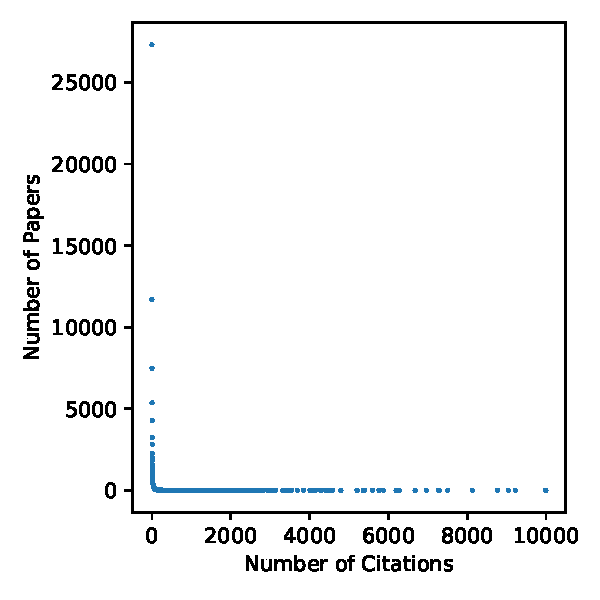
\includegraphics[width=\textwidth]{images/s2_dist.pdf}
    \end{minipage}%
    \begin{minipage}{0.48\textwidth}
        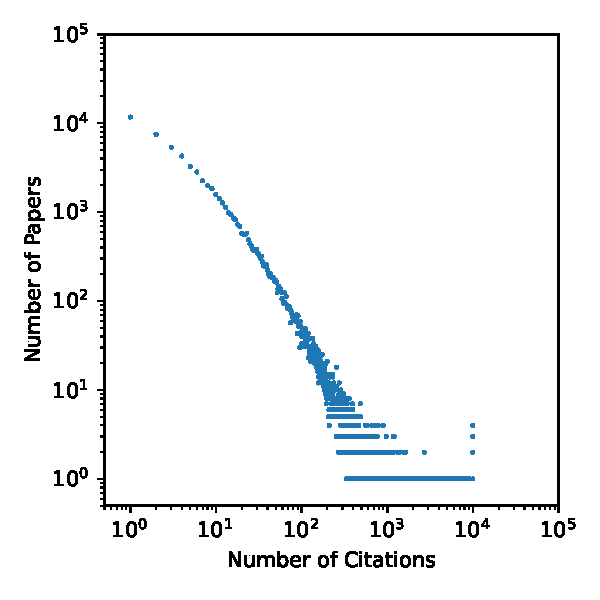
\includegraphics[width=\textwidth]{images/s2_dist_log.pdf}
    \end{minipage}
    \caption{Citation number follows a power-law distribution according to S2.
    (Left): Normal scale. (Right): Log-log scale excluding the zero-cited papers.}
    \label{fig:s2_dist}
\end{figure}

We use the S2 citation numbers to filter out highly citated papers.
We keep 4,422 papers with S2 citation numbers larger than or equal to 100 as the highly cited papers.

The second data source is Google Scholar.
Google Scholar also provides citation numbers on its website.
However, it does not support API retrival due to unspecified reasons.
Getting citation numbers from Google Scholar can only be done semi-automatically.

The use of two data sources has both strengths and limitations,
so we ensemble two parts together by taking the mean of the two.
Fig. \ref{fig:distribution} shows the distribution of the highly cited papers.
\footnote{Raw metadata of the 4,422 papers can be downloaded at: \url{http://star-lab.ai/arxiv/arxiv_4422.tar.gz}}

\begin{figure}
    \centering
    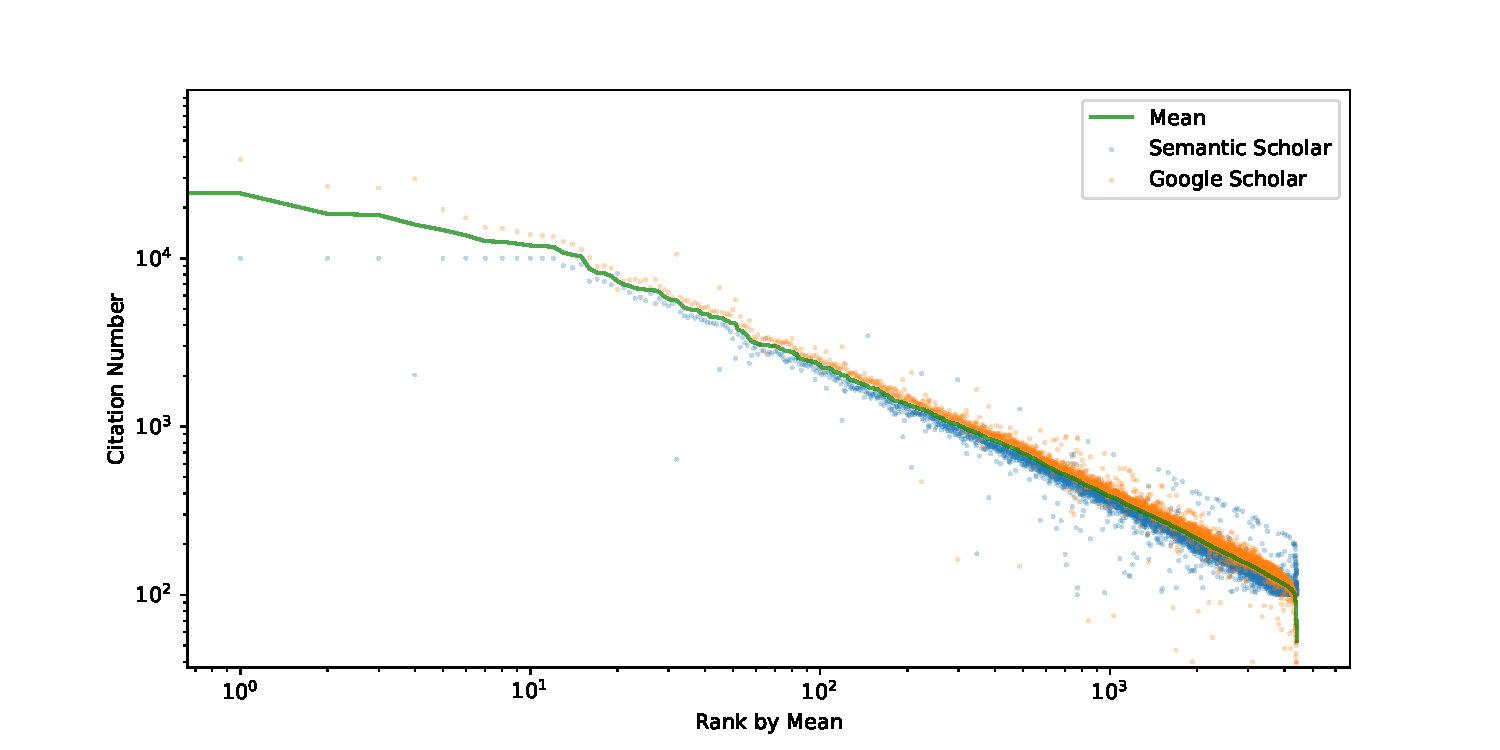
\includegraphics[width=\textwidth]{images/citation_number_distribution.pdf}
    \caption{Citation number distribution for highly cited 4,422 arXiv cs.LG and cs.AI papers.
        The blue dots are the Semantic Scholar citation numbers ($S2$),
        and the orange dots are the Google Scholar citation numbers ($GS$).
        For most of the papers, $GS$ are higher than $S2$.
        $S2$ are bounded by $10^4$, which might due to their system limitation.
        But $GS$ misses some papers which $S2$ consider them as highly cited.
        The green line is the mean of $S2$ and $GS$.
    }
    \label{fig:distribution}
\end{figure}

\subsection{Relationship Between Papers}

Now we have 4,422 highly cited papers.
We define a undirected weighted network $G(V,E)$, with its nodes set $V$ to be the set of those papers, and its edges set $E$ to be the set of the relationships between papers.

Our objective is to reveal the structure of the research community.
Based on this objective, we define the weights $w_{i,j}$ of the edge between papers based on the overlaps in authorships.
We divide the authors of a paper into two classes: ($A$) the first author and the last author, ($B$) other authors which are neither the first nor the last author.

There are multiple inconsistencies in arXiv metadata and Semantic Scholar metadata, we tried to correct some errors, but still there are remaining ones.
In this case, we use the metadata from arXiv.

Class ($A$) always at least contains one author, and class ($B$) could be empty if there are no other authors.
We give a weight of 1.0 if class ($A$) of two papers overlap.
Otherwise, we give a weight of 0.5 if class ($A$) of one paper overlaps with ($B$) of another paper.
Otherwise, we give a weight of 0.3 if class ($B$) of two papers overlap.

This is an ad hoc method to define the relationships.
One can come up with other definitions and the pipeline will still work.

Fig. \ref{fig:matrix_random_arrangement} shows the adjacent matrix of the constructed network $G$ with a random arrangement (which is almost blank).

\begin{figure}
    \centering
    
\includegraphics[width=\textwidth]{images/random_arrangement.png}
    \caption{The relationship matrix in a random arrangement before matrix reordering.
        Dark grids mean they have values, which represent the author relationships between two papers.
        The diagonal line is defined to be 1.0.
        However, a 4422x4422 matrix with a random arrangement is almost meaningless to a human observer.
        (The image looks almost blank due to the sparsity of the matrix.)
    }
    \label{fig:matrix_random_arrangement}
\end{figure}
